\section{ĐƯỜNG THẲNG VÀ MẶT PHẲNG SONG SONG}
\subsection{KIẾN THỨC CẦN NHỚ}
\subsubsection{VỊ TRÍ TƯƠNG ĐỐI CỦA ĐƯỜNG THẲNG VÀ MẶT PHẲNG}
Cho đường thẳng $a$ và mặt phẳng $(P) $. Căn cứ vào số điểm chung của đường thẳng và mặt phẳng, ta có ba trường hợp sau:\\
\begin{tabular}{lll}
	\begin{tikzpicture}[scale=.8]
		\tkzDefPoints{0/0/A', 4/0/B', 1/2/D', 0/2.5/M}
		\coordinate (C') at ($(B')+(D')-(A')$);
		\tkzDefPointBy[translation = from A' to B'](M) \tkzGetPoint{N}
		\tkzLabelSegment[pos=.3](M,N){ $a$}
		%\tkzDrawSegments[dashed](A,A' A',B' A',C')
		\tkzDrawPolygon(A',B',C',D')
		\tkzDrawSegments(M,N)
		%\tkzLabelPoints[right](B)
		%\tkzLabelPoints[above](z,y)
		\tkzMarkAngles[size=1](B',A',D')
		\tkzLabelAngle[pos=0.6](D',A',B'){\footnotesize $P$ }
		%\tkzDrawPoints(M,N,A)
	\end{tikzpicture}
	&\begin{tikzpicture}[scale=.8]
		\tkzDefPoints{0/0/A', 4/0/B', 1/2/D', 2/1/A, 0/2.5/B}
		\coordinate (C') at ($(B')+(D')-(A')$);
		\tkzLabelSegment[pos=.3](A,B){ $a$}
		\tkzInterLL(A,B)(A',B')\tkzGetPoint{I}
		\tkzInterLL(A,B)(C',B')\tkzGetPoint{J}
		\tkzDrawPolygon(A',B',C',D')
		\tkzDrawSegments(A,B I,J)
		\tkzDrawSegments[dashed](A,I)
		%\tkzLabelPoints[right](B)
		\tkzLabelPoints[above right](A)
		\tkzMarkAngles[size=1](B',A',D')
		\tkzLabelAngle[pos=0.6](D',A',B'){\footnotesize $P$ }
		\tkzDrawPoints(A)
	\end{tikzpicture}
	&\begin{tikzpicture}[scale=.8]
		\tkzDefPoints{0/0/A', 4/0/B', 1/2/D', 1/1/A, 4/1/B}
		\coordinate (C') at ($(B')+(D')-(A')$);
		\tkzLabelSegment[pos=.6](A,B){$a$}
		%\tkzDrawSegments[dashed](A,A' A',B' A',C')
		\tkzDrawPolygon(A',B',C',D')
		\tkzDrawSegments(A,B)
		%\tkzLabelPoints[right](B)
		\tkzLabelPoints[above](A,B)
		\tkzMarkAngles[size=1](B',A',D')
		\tkzLabelAngle[pos=0.6](D',A',B'){\footnotesize $P$ }
	\end{tikzpicture}\\
	\small * $a$ và $(P)$ không có điểm chung.  & \small * $a$ và $(P)$ có đúng 1 điểm chung. & \small * $a$ và $(P)$ có vô số điểm chung.\\
	\small * $a$ song song $(P)$. Kí hiệu $a \parallel (P)$. & \small * $a$ cắt $(P)$. Kí hiệu $a \cap (P)=A $.  & \small * $a$ nằm trong $(P)$. Kí hiệu 	$a \subset (P)$.
\end{tabular}

\subsubsection{CÁC ĐỊNH LÝ VÀ HỆ QUẢ CẦN NHỚ}
\begin{enumerate}[\iconMT]
	\immini{\item \indam{Định lý 1:} Nếu đường thẳng $a$ không nằm trong mặt phẳng $(P)$ và song song với một đường thẳng nào đó trong $(P)$ thì $a$ song song với $(P)$, hay
	$$a\not\subset (P) \text{ và } \heva{&a\parallel d \\&d\subset (P)\\}\Rightarrow a\parallel (P)$$}{\hspace{1cm}
	\begin{tikzpicture}[scale=0.57]
		\tkzDefPoints{0/0/A', 4/0/B', 1/2/D', 1/1/A, 4/1/B, 0/2.5/M}
		\coordinate (C') at ($(B')+(D')-(A')$);
		\tkzDefPointBy[translation = from A' to B'](M) \tkzGetPoint{N}
		\tkzLabelSegment[pos=.3](M,N){ $a$}
		\tkzLabelSegment[pos=.3](A,B){ $d$}
		%\tkzDrawSegments[dashed](A,A' A',B' A',C')
		\tkzDrawPolygon(A',B',C',D')
		\tkzDrawSegments(A,B M,N)
		%\tkzLabelPoints[right](B)
		%        \tkzLabelPoints[above](A,B)
		\tkzMarkAngles[size=0.8](B',A',D')
		\tkzLabelAngle[pos=0.5](D',A',B'){\footnotesize $P$ }
	\end{tikzpicture}
}
	\immini{
		\item \indam{Định lý 2:}Cho hai đường thẳng chéo nhau. Có duy nhất một mặt phẳng chứa đường thẳng này và song song với đường thẳng kia.
	}{	\begin{tikzpicture}[>=stealth,scale=0.45, line join=round, line cap=round]
	\tikzset{label style/.style={font=\footnotesize}}
	\tkzDefPoints{0/0/A, 6/0/B, 5/-3/C, -1/-3/D, 1/-1/E, 5/-1/b', 4/-2.5/a, 2/-1/M, 1/-0.5/Q, 1/1/L, 5/1/b}	
	\tkzDrawSegments(A,B B,C C,D D,A E,b' a,Q L,b)		
	\tkzLabelPoints[above](M,b',b,a)	
	\tkzMarkAngles[size=0.8cm](C,D,A)
	\tkzLabelAngles[pos=0.5,rotate=30](C,D,A){\scriptsize$\alpha$}
\end{tikzpicture}}
	\immini{\item \indam{Định lý 3:} Nếu đường thẳng $a$ song song với mặt phẳng $(\alpha)$. Nếu mặt phẳng $(\beta)$ chứa $a$ và cắt $(\alpha)$ theo giao tuyến $b$ thì $b$ song song với $a$.}{
	\begin{tikzpicture}[>=stealth,scale=0.46, line join=round, line cap=round]
		\tikzset{label style/.style={font=\footnotesize}}
		\tkzDefPoints{0/0/A,6/0/B, 4/-2/C,-2/-2/D,1/0/I, 4/0/J, 5/-1/L, 2/-1/M, 2/2/H, -1/2/K, 0.5/1/E, 2.5/1/F, 2/1/a, 3/-1/b}	
		\tkzDrawSegments(A,I J,B B,C C,D D,A M,K L,H H,K E,F)
		\tkzDrawSegments[thick,blue](M,L)
		\tkzDrawSegments[dashed](I,J)
		\tkzLabelPoints[above](a,b)	
		\tkzMarkAngles[size=0.8cm](C,D,A)
		\tkzLabelAngles[pos=0.5,rotate=30](C,D,A){\scriptsize $\alpha$}
		\tkzMarkAngles[size=1cm](M,K,H)
		\tkzLabelAngles[pos=0.6,rotate=340](M,K,H){\scriptsize $\beta$}
\end{tikzpicture}}
\immini{
	\begin{luuy}
		Nếu hai mặt phẳng phân biệt cùng song song với một đường thẳng thì giao tuyến của chúng (nếu có) cũng song song với đường thẳng đó.
	\end{luuy}
}{	\begin{tikzpicture}[>=stealth,scale=0.46, line join=round, line cap=round]
		\tikzset{label style/.style={font=\footnotesize}}
		\tkzDefPoints{0/0/A, 4/0/B, 4/5/C, 0/5/D, 2/4/E, 2/0/I, 2/-1/F, 5/4/M, 5/-1/N, 0/2/d', 5/2/d}	
		\tkzDrawSegments(A,D  A,F  F,E  E,D  I,B  B,C  C,D  M,N)
		\tkzDrawSegments[dashed](A,I)
		\tkzLabelPoints[right](d)	
		\tkzLabelPoints[left](d')
		\tkzMarkAngles[size=0.8cm](E,F,A)
		\tkzLabelAngles[pos=0.5,rotate=30](E,F,A){\scriptsize $\alpha$}
		\tkzMarkAngles[size=0.8cm](C,B,A)
		\tkzLabelAngles[pos=0.5,rotate=30](C,B,A){\scriptsize $\beta$}
\end{tikzpicture}}	
\end{enumerate}

\begin{dang}{Chứng minh đường thẳng song song với mặt phẳng}
	\begin{enumerate}[\iconMT]
		\item \indam{Phương pháp giải:} Để chứng minh đường thẳng $a$ song song với mặt phẳng $(P)$, ta cần chứng tỏ các ý sau đây
		\immini{
			\begin{itemize}
				\item [$\bullet$] $a$ không nằm trên $(P)$;
				\item [$\bullet$] $a$ song song với một đường thẳng $b$ nằm trong $(P)$. Suy ra $a\parallel (P)$.
				\item [] Tóm lại \quad \quad \fbox{$\heva{&a\not\subset (P)\\&a\parallel b \\&b\subset (P)\\}\Rightarrow a\parallel (P)$}
			\end{itemize}
		}{\vspace{1cm}
			\begin{tikzpicture}[scale=0.7]
				\tikzset{label style/.style={font=\footnotesize}}
				\tkzDefPoints{0/0/A', 4/0/B', 1/2/D', 1/1/A, 4/1/B, 0/2.5/M}
				\coordinate (C') at ($(B')+(D')-(A')$);
				\tkzDefPointBy[translation = from A' to B'](M) \tkzGetPoint{N}
				\tkzLabelSegment[pos=.3](M,N){ $a$}
				\tkzLabelSegment[pos=.3](A,B){ $d$}
				%\tkzDrawSegments[dashed](A,A' A',B' A',C')
				\tkzDrawPolygon(A',B',C',D')
				\tkzDrawSegments(A,B M,N)
				%\tkzLabelPoints[right](B)
				%        \tkzLabelPoints[above](A,B)
				\tkzMarkAngles[size=0.8](B',A',D')
				\tkzLabelAngle[pos=0.5](D',A',B'){\footnotesize $P$ }
		\end{tikzpicture}}
		\item \indam{Chú ý:} Việc chứng minh $a \parallel b$, ta thường đi đến việc xét các yếu tố song song đã biết trong hình học phẳng như
		\immini{\begin{listEX}[1]
				\item [\ding{172}] Cặp cạnh đối của hình bình hành;
				\item [\ding{173}] Đường trung bình trong tam giác;
				\item [\ding{174}] Tỉ lệ $\dfrac{AM}{AB}=\dfrac{AN}{AC}\Rightarrow MN \parallel BC$ (hình bên). Đặc biệt cần chú ý tỉ lệ trọng tâm của tam giác.
			\end{listEX}
		}{
			\begin{tikzpicture}[scale=0.8, line join=round, line cap=round]
				\tkzDefPoints{0/0/B,5/0/C,1.5/2/A}
				\coordinate (M) at ($(A)!0.3!(B)$);
				\coordinate (N) at ($(A)!0.3!(C)$);
				\tkzDrawPoints[size=5,fill=black](A,B,C,M,N)
				\tkzDrawSegments(M,N)
				\tkzDrawPolygon(A,B,C)
				\tkzLabelPoints[below,font=\footnotesize](B,C)
				\tkzLabelPoints[above,font=\footnotesize](A)
				\tkzLabelPoints[left,font=\footnotesize](M)
				\tkzLabelPoints[right,font=\footnotesize](N)
		\end{tikzpicture}}
	\end{enumerate}
\end{dang}

\begin{dang}{Tìm giao tuyến của hai mặt phẳng cắt nhau}
	\begin{enumerate}[\iconMT]
		\item \indam{Các phương pháp đã học ở hai bài trước:}
		\begin{listEX}[1]
			\item [\ding{172}] Tìm hai điểm chung phân biệt. Khi đó giao tuyến là đường thẳng đi qua hai điểm chung đó.
			\item [\ding{173}] Nếu hai mặt phẳng lần lượt chứa hai đường thẳng song song thì giao tuyến của chúng (nếu có) cũng song song hoặc trùng với một trong hai đường thẳng đó.
		\end{listEX}
		\item \indam{Ta xét thêm một trong hai cách sau:}
		\begin{listEX}[1]
			\item [\ding{172}] Nếu đường thẳng $a$ song song với mặt phẳng $(\alpha)$ và mặt phẳng $(\beta)$ chứa $a$ và cắt $(\alpha)$ theo giao tuyến $b$ thì $b$ song song với $a$.\\
			hay \quad \quad  \fbox{$\heva{&a\parallel (\alpha)\\&a\subset (\beta) \\&M\in (\alpha)\cap (\beta)}\Rightarrow (P)\cap (\beta) =Mx \parallel a$}
			\item [\ding{173}] Nếu hai mặt phẳng phân biệt cùng song song với một đường thẳng thì giao tuyến của chúng (nếu có) cũng song song với đường thẳng đó.\\
			hay \quad \quad \fbox{$\heva{&a\parallel (\alpha)\\&a\parallel (\beta)\\&M\in (\alpha)\cap (\beta)}\Rightarrow (\alpha)\cap (\beta) =Mx\parallel a$}.
		\end{listEX}
	\end{enumerate}
\end{dang}		
	
